\documentclass{standalone}
\usepackage{tikz}
\usepackage{ctex,siunitx,ninecolors}
\setCJKmainfont{Noto Serif CJK SC}
\usepackage{tkz-euclide}
\usepackage{amsmath}
\usetikzlibrary{patterns, calc}
\usetikzlibrary {decorations.pathmorphing, decorations.pathreplacing, decorations.shapes,}
\begin{document}
\small
\begin{tikzpicture}[>=stealth,scale=1.0]
  \node at(-7.5,0) {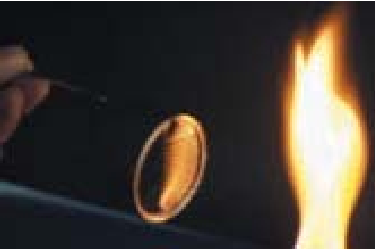
\includegraphics[height=2.7cm]{a.pdf}};
  \draw[cyan,domain=-3:0,samples=200] plot (\x, {0.2*sin(\x*2*pi r)});
  \draw[cyan,densely dashed,domain=-3:0,samples=200] plot (\x, {-0.2*sin(\x*2*pi r)});
  \draw[cyan,domain=-3:0,samples=200] plot (\x, {0.2*sin(\x*2*pi r)+1.5});
  \draw[cyan,densely dashed,domain=-3:0,samples=200] plot (\x, {0.2*sin(\x*2*pi r)+1.45});
  \draw[cyan,domain=-3:0,samples=200] plot (\x, {0.2*sin(\x*2*pi r)-1.5});
  \draw[cyan,densely dashed,domain=-3:0,samples=200] plot (\x, {0.2*sin(\x*2*pi r)-1.55});
  \fill[cyan!40!white](-0.4,2)--(-0.8,-2)--(0.8,-2)--(0.4,2)--cycle;
  \node at (-3.5,1.5){亮};
  \node at (-3.5,0){暗};
  \node at (-3.5,-1.5){亮};
  \draw (0,1.2)--++(30:0.8)node[right]{肥皂液膜};
\end{tikzpicture}
\end{document}